\documentclass[]{article}
\usepackage{upquote}
\usepackage{listings}
\usepackage{color}
\usepackage[margin=1cm]{geometry}
 \usepackage{graphicx}
\usepackage[section]{placeins}
\usepackage{url}
%\usepackage{wrapfig}
\begin{document}

\title{NewzTrader: Autonomous Trading Agent Implementation Using Natural Language Processing Of News Headlines}
\author{William Lyon}
\date{\today}
\maketitle
\abstract{\noindent Natural Language Processing techniques are used to examine financial news headlines and generate predictions of stock price movements.  News headlines from the Wall Street Journal from January 1, 2009 to November 1, 2012 are collected and paired with daily S\&P 500 index returns.  This information is used to train a text classifier and generate BUY/SELL trading signals.  This simple trading strategy is then backtested using Wall Street Journal news headlines as a predictor for movement in the price of the S\&P 500 index. }

\section{Introduction}
In finance, the Efficient Market Hypothesis states that all publicly available information is reflected in financial market prices.  As new information becomes available, prices adjust to take this new information into account.  In accordance with the Efficient Market Hypothesis, financial news should directly influence stock price movements as the news items become publicly available.  This paper uses financial news headlines to train a machine-learning agent to predict short term fluctuations in the value of the S\&P 500 stock market index.  Naive Bayes and Maximum Entropy classifiers are built and used to classify news headlines as indicative of an increase, decrease, or no movement of the value of the S\&P 500 index (within a 1\% threshold).  These classifiers are then used to generate Buy and Sell trading signals and this trading strategy is backtested by trading against the S\&P 500 index.     
\subsection{Motivation}
This tool could be used as a component of an autonomous trading agent that will make BUY/SELL decisions for trading financial instruments.  An autonomous trading agent is more likely to be effective if buy/sell signals are generated by an ensemble model, where the ultimate buy/sell signal is taken by polling many independent predictive models and combining a weighted average of predictions \cite{barbosa08}.  Therefore it should not be expected that the Natural Language Processing component alone should be profitable during backtesting.  
\subsection{Literature Review}
Daskalopoulos 2003 presents a method of predicting short term stock price fluctuations of individual company stocks by classifying company-specific news headlines using a Naive Bayes classifier\cite{dask03}.  He reports accuracy of between 0.988 and 0.945.  However, the threshold for identifying a RISE or FALL instance is set at a one day change in the stock price of 10\%, which is very rare.  In fact, he indicates the prior probability of a NOTHING instance (a daily stock return of between -9.99\% and 9.99\%) is 0.978.  Thus a classifier that only predicts NOTHING classes would have accuracy of 0.978. Skiena, et al. 2010 uses a more complicated sentiment analysis approach and wider selection of text data (including blogs, Twitter, and daily newspapers) to predict individual stock price movements and evaluates the model using trading backtesting.  The paper finds their approach to have consistent returns over the course of five years of backtesting\cite{skiena10}. 
\subsection{Initial Attempt}
Initially I set out with the goal of duplicating Daskalopoulos's\cite{dask03} results and building on that by using trading backtesting to further evaluate the model.  I collected stock specific data by using a Google Finance API which returned an XML document listing news headlines relevant to a specific company.  After building a Naive Bayes classifier using the company specific news headlines, accuracy was unfortunately quite low: around 0.10 on average.  I believe these poor results relative to Daskalopoulos can be explained by 1) using a lower threshold for identifying UP/DOWN/NONE classes and 2) removal of news items from Google Finance.  I chose to use a much lower threshold for identifying UP/DOWN/NONE instances than Daskalopoulos (+/- 3\% vs. +/- 10\% daily returns).  Since daily returns exceeding 10\% absolute value are quite rare, a trading strategy using this model would be quite ineffective.  Also, it appears Google for some reason removes news items from Google Finance after a relatively short period of time.  Therefore the same data contained many recent news items but few news items dating beyond one year.  This made building a multi-year collection of test data difficult.  After this initial setback I moved to the model described below.
\section{The Data}
For this experiment news headlines and stock quotes from Jan 1, 2009 to Nov 1, 2012 were collected.  News headlines were limited to the Wall Street Journal Business section.  Stock quotes were daily open, low, high, and close of the S\&P 500 index.
\subsection{Historical Stock Market Quotes}
Historical stock price data is available from Yahoo! Finance and was downloaded using the Python pandas data analysis library, which includes a method for importing Yahoo! Finance data directly into a pandas object.  The S\&P 500 index was chosen because it is a broad market index that incorporates companies from all major industries and is a good proxy for the market as a whole.  Daily quotes were collected, however quotes of higher frequency (hourly, 15-minute, etc.) would have been preferred and would more accurately reflect how a trading system such as NewzTrader would perform in a real trading environment.  Unfortunately stock quote data in frequency greater than daily is more difficult to obtain and expensive.  For the purposes of this initial experiment daily quotes are acceptable, but it should be noted that higher frequency data is ideal.
\subsection{News Headlines}
Wall Street Journal Business section news headlines were collected using an API provided by NewsCred \cite{newscred}.  NewsCred is a company that provides access to full-text news articles, including The Wall Street Journal.  A limited-use API key was provided by NewsCred, which allowed for access to headlines only.  The NewsCred API was used to retrieve daily Wall Street Journal news headlines, which were then limited to articles tagged by NewsCred as belonging to the "Business" category.  A total of 101,618 news headlines over 1416 days were collected with an average of 71 headlines per day.  
\subsection{Initial Data Exploration}
Each news headline's publication date was aligned with the S\&P 500 stock quote for that date.  Headlines were removed from the corpus if no stock quote was available for that day (non-trading day, missing data, etc.). After aligning with stock quote data, a total of 85,775 news headlines remained in the corpus.  These were stored in a dictionary data structure where the key corresponded to a date and the values were a list of the news headlines for that date.  The corpus of news headlines consisted of a total of 199,511 words.  Figure 1 shows a cumulative frequency plot of the 50 most common words in the news headline corpus.
\begin{figure}
%\begin{wrapfigure}{o}{8cm}
\centering
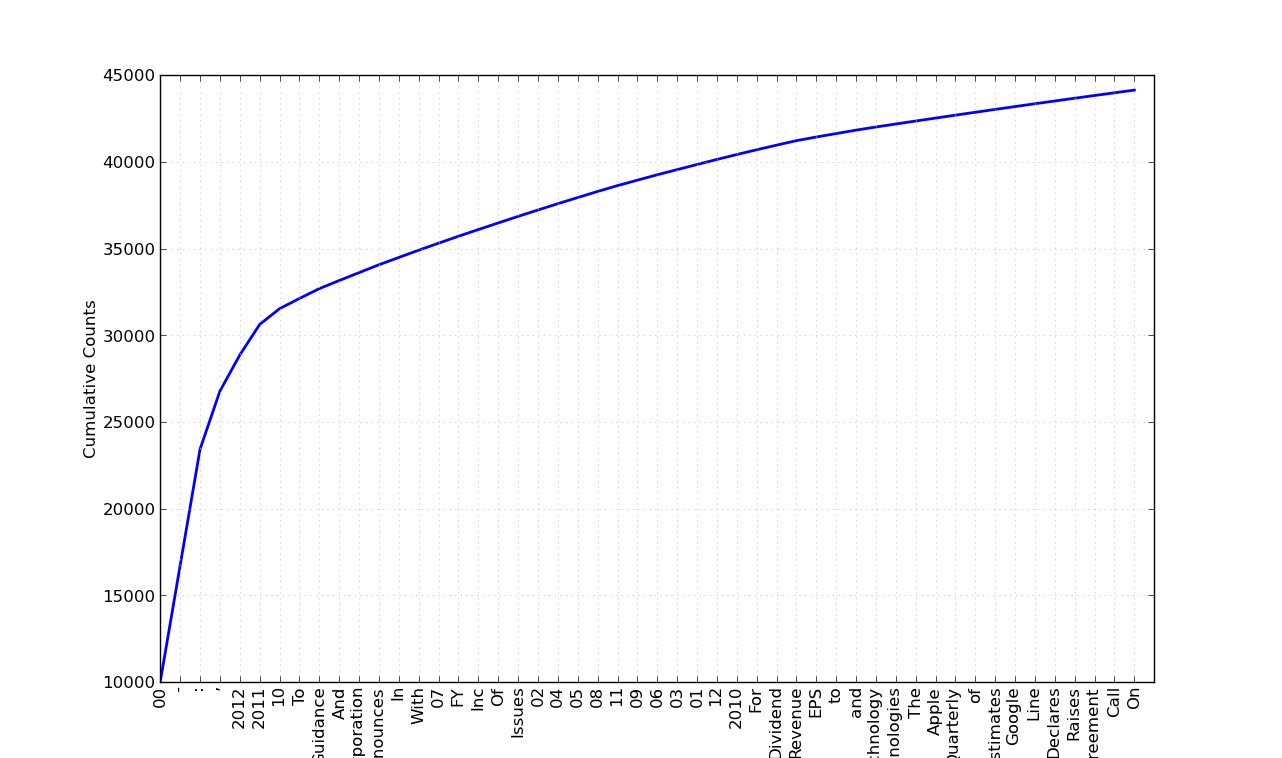
\includegraphics[scale=0.25]{cum_graph.png}
\caption{Cumulative frequency plot}
\end{figure}
%\end{wrapfigure}
%\end{figure}
%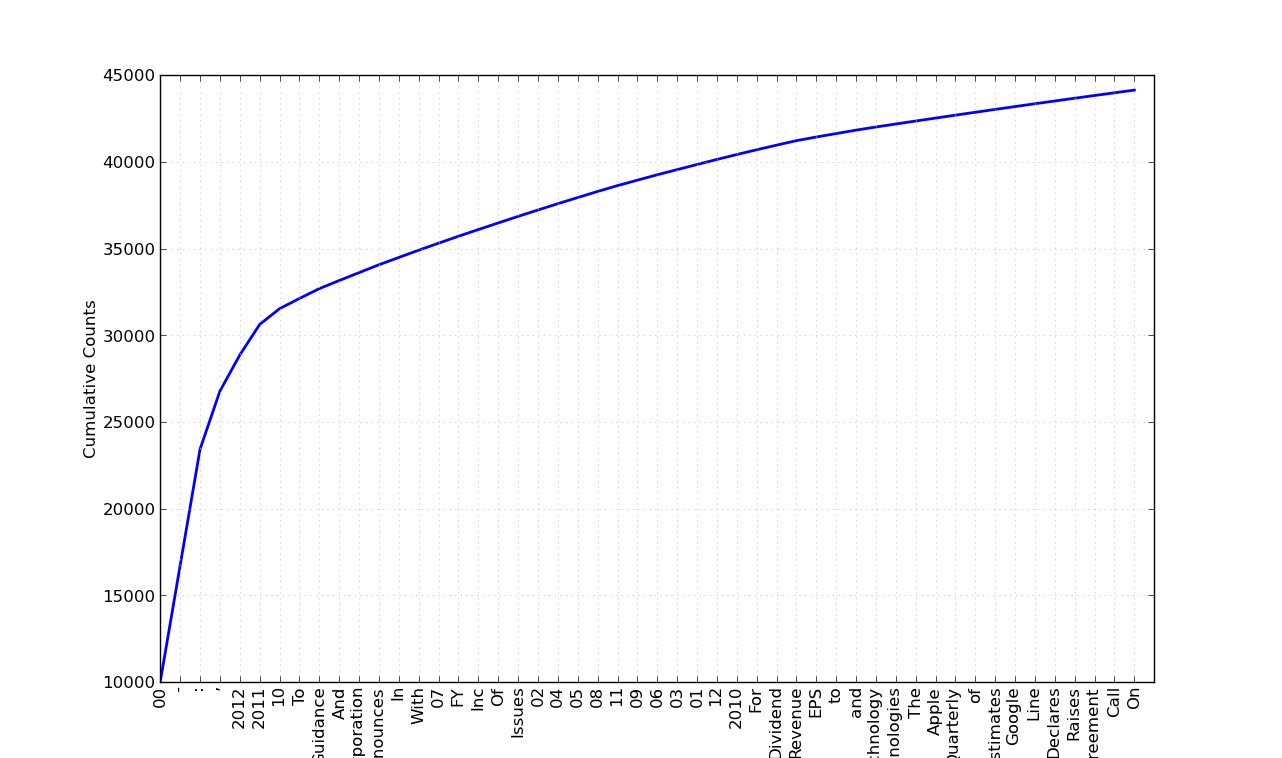
\includegraphics[width=60mm]{cum_graph.png}
%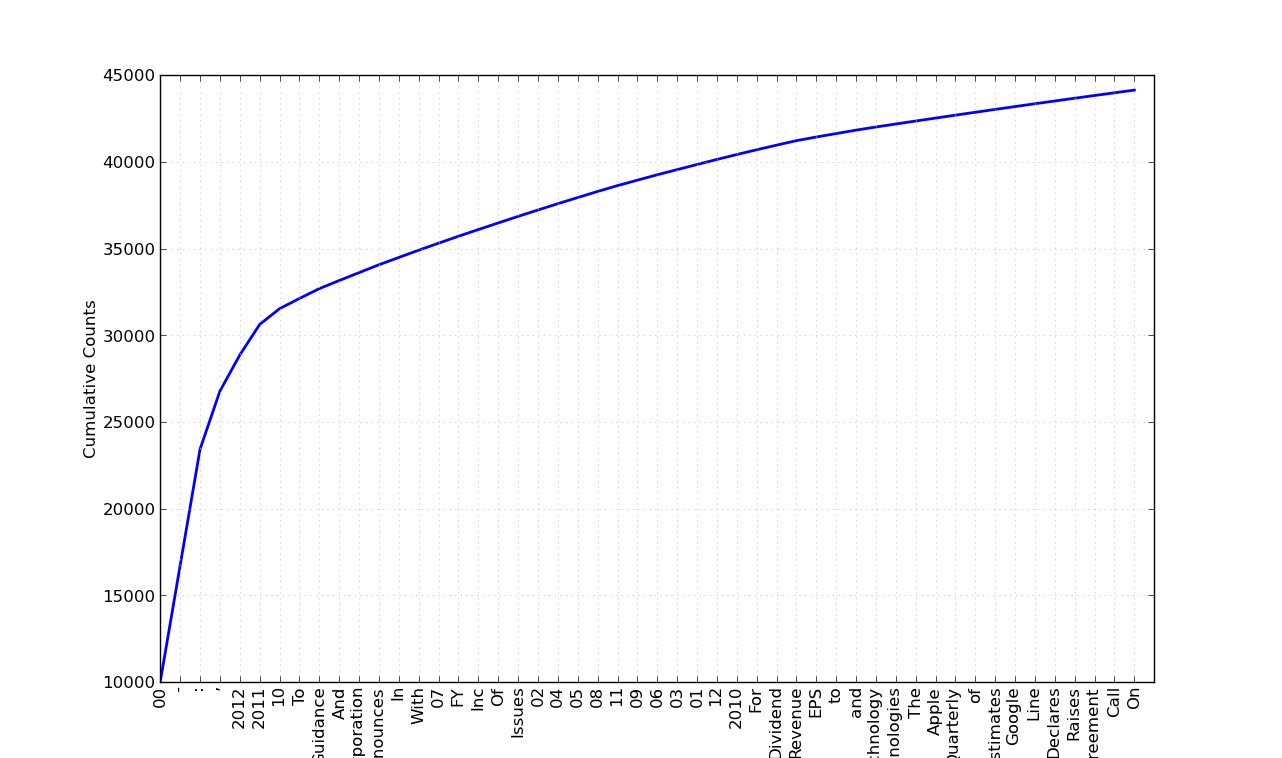
\includegraphics[height=60mm]{cum_graph.jpg}
%\includegraphics[scale=0.75]{myfig.pdf}
%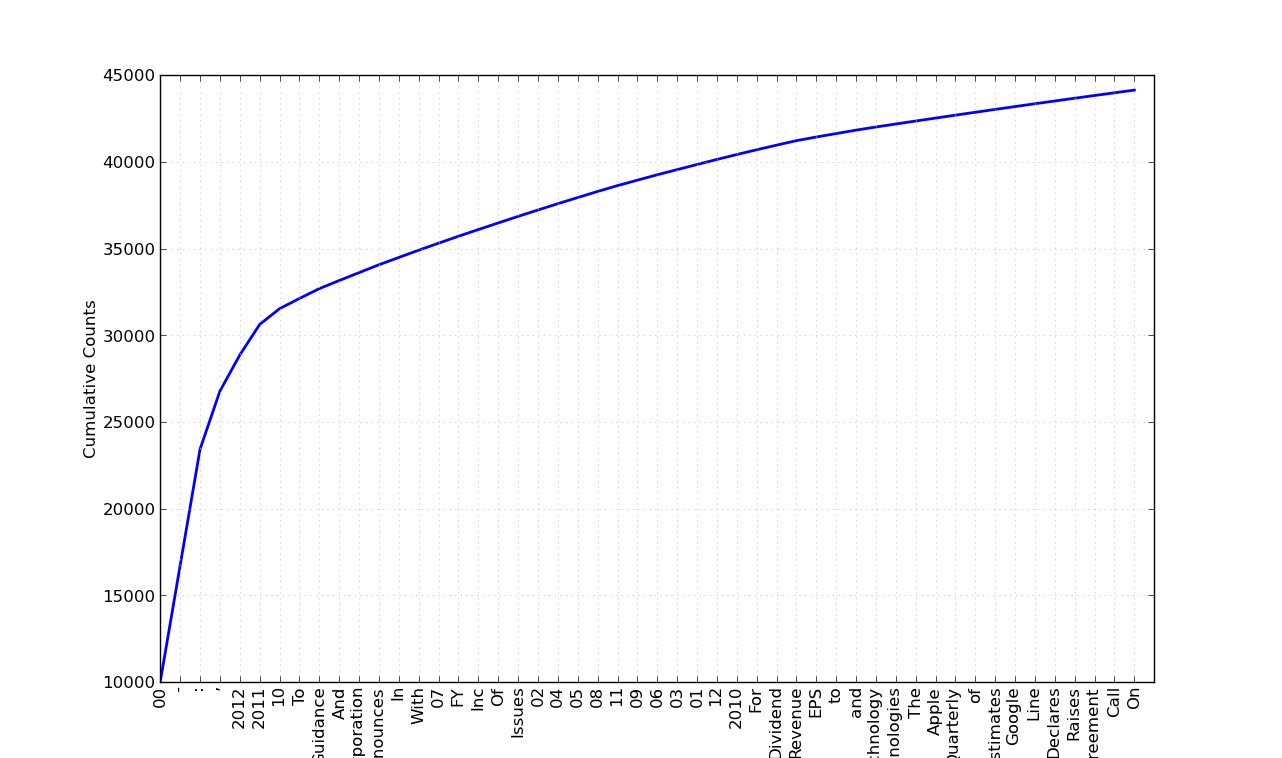
\includegraphics[angle=45,width=52mm]{cum_graph.png}
\section{Classification Methodology}
Every observed trading day was classified as either UP, DOWN, or NONE depending on the return of the S\&P 500 index for that day, relative to the previous trading day, using a threshold of 1.5\% of the previous day's value.  Days where the S\&P 500 closed at least 1.5\%  higher than the previous day's close were classified as UP.  Days where the S\&P500 close was at least 1.5\% lower than the previous day's close were classified as DOWN.  Days closing within 1.5\% were classified as NONE.  The distribution of classifications were as follows:
UP: 14651
DOWN: 13718
NONE: 57405
TOTAL: 85775.
Resulting in the following prior probabilities: 
UP: 0.1708
DOWN: 0.1599
NONE:  0.6693.
These tuples of  \{classification, listOfNewsHeadlines\} were used as the training data for a Naive Bayes classifier and a Maximum Entropy classifier.  The Python Natural Language Toolkit (NLTK) was used for handling text processing as well as the built-in classifiers. 
\subsection{Naive Bayes}
Summarize NB from NLTK book
\subsection{Maximum Entropy}
Summarize ME from NLTK book

\section{Implementation}

\subsection{Dependencies}
Several Python packages are required to run NewzTrader.  The required packages and their purpose are described below.
\begin{description}
 
\item[NLTK] The Python Natural Language Toolkit is used for text processing, as well as the built-in classifiers Naive Bayes and Maximum Entropy. 

\item[pandas] Data analysis library
\item[LXML] Used for parsing XML
\item[Dateutil] Used for parsing date strings
\item[Matplotlib] Used for plotting
\item[Zipline] Financial backtesting library used for backtesting of NewzTrader
\item[Numpy] Numeric Python library

\end{description}
\subsection{Data Collection \& Munging - newsCredScraper.py}
\subsection{Training NLP Classifier - }
\subsubsection{Bag of words}
\subsubsection{Filtering stopwords}
\subsubsection{Include significant bigrams}
\subsection{Naive Bayes Classifier}
\subsection{Maximum Entropy Classifier}
\subsection{Backtesting}
\section{Evaluation}

\begin{table}[h]
\centering
\begin{tabular}{| c | c | c | c | c | c|c|c|}
\hline
Classifier & Accuracy & Recall(NONE) &Recall(UP)&Recall(DOWN)&Precision(NONE)&Precision(UP)&Precision(DOWN)\\
\hline
NB-full & 0.48 & 0.5814 & 0.3076 & 0.2945 & 0.7054 & 0.2292 & 0.2150\\
\hline
NB-0910 & 0.45 & 0.5361 & 0.3110 & 0.2947 & 0.6695 & 0.2374 & 0.2151\\
\hline
ME-full & 0.6680 & 0.9335 & 0.1139 & 0.1035 & 0.6883 & 0.3857 & 0.3944\\
\hline
ME-0910 & 0.6155 & 0.9499 & 0.0439 & 0.0503 & 0.6374 & 0.2636 & 0.3025 \\
\hline

\end{tabular}
\caption{Evaluation metrics. NB-full=Naive Bayes, full data; NB-0910=Naive Bayes 2009-2010 data only; ME-full=Maximum Entropy, full data; ME-0910=Maximum Entropy 2009-2010 data only}
\end{table}

\begin{table}
\centering
\begin{tabular}{|c|c|c|}
\hline
& Naive Bayes & Maximum Entropy\\
\hline
Accuracy & 0.6381& 0.4091\\
\hline
Recall(NONE) & 0.9594 & 0.4698\\
\hline
Recall(UP) & 0.0929 & 0.5161 \\
\hline
Recall(DOWN) & 0.0908 &  0.0782 \\
\hline
Precision(NONE) & 0.6508 & 0.6288 \\
\hline
Precision(UP) & 0.5035  & 0.1996 \\
\hline
Precision(DOWN) & 0.4452 & 0.4375 \\
\hline

\end{tabular}
\caption{Evaluation metrics, high information words only for 2009-2010 data only}
\end{table}

\subsection{Accuracy}


\subsection{Precision}

\subsection{Recall}
\subsection{Most informative features}
\section{Trading Model}
\subsection{Trading Signals}
\subsection{Backtesting}
\begin{figure}
%\begin{wrapfigure}{o}{8cm}
\centering
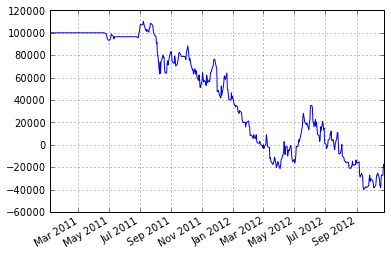
\includegraphics[scale=0.6]{paper/img/backtestPortValue.png}
\caption{Portfolio value with backtesting strategy}
\end{figure}

This is the backtestinfg. Where is the rest of the backtesting?
\begin{figure}
%\begin{wrapfigure}{o}{8cm}
\centering
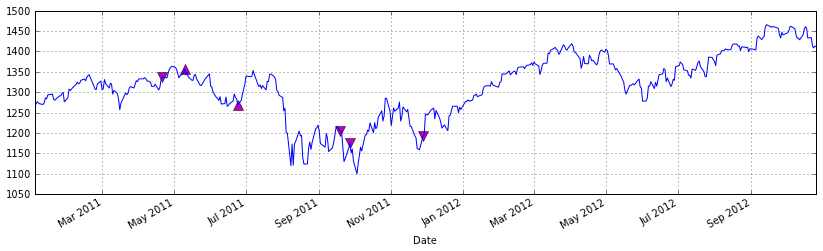
\includegraphics[scale=0.6]{paper/img/backtestNB.png}
\caption{Backtest buy/sell signals}
\end{figure}

\section{Conclusions}
In backtesting, the trading strategy tested by NewzTrader is not profitable.  This can be attributed to the relatively low accuracy of the classifier and specifically the very low recall measures of the UP and DOWN classifications.  

\subsection{Further research}



\begin{thebibliography}{9}

\bibitem{bird09}
  Steven Bird, Ewan Klein, and Edward Loper,
  \emph{Natural Language Processing with Python}.
  O'Reilly Media Inc, California
  1st Edition,
  2009.

\bibitem{perkins10}
  Jacob Perkins,
  \emph{Python Text Processing with NLTK 2.0 Cookbook}.
  Packt Publishing, Birmingham, UK
  1st Edition,
  2010

\bibitem{dask03}
  Daskalopoulos, V,
  \emph{Stock Price Prediction From Natural Language Understanding of News Headlines}.
  Presented at Information Conference on Machine Learning (iCML03), 2003. 
  \url{http://www.cs.rutgers.edu/~mlittman/courses/ ml03/iCML03/papers/daskalopoulos.pdf.}

\bibitem{peram02}
  Peramunetilleke, D. et al., 
  \emph{Currency Exchange Rate Forecasting From News Headlines}.
  Australian Computer Science Communications.
  Vol 24:2 Jan-Feb 2002,
  pp131-139.

\bibitem{barbosa08}
  Barbosa, R., et al.,
  \emph{Algorithmic Trading Using Intelligent Agents}.
  2008 International Conference on Image Processing, Computer Vision, and Pattern Recognition.

\bibitem{skiena10}
  Skiena, S. et al.,
  \emph{Trading Strategies To Exploit Blog and News Sentiment}.
  Fourth International Conference on Weblogs and Social Media 2010,
  Washington, DC, May 23-26, 2010. 
  \url{http://www.cs.sunysb.edu/~skiena/lydia/blogtrading.pdf}

\bibitem{newscred}
\url{http://newscred.com/developer/docs/module/article/doc}

\end{thebibliography}
\section{Source Code Listings}

\lstset{frame=shadowbox, numbers=left, float, caption=newsCredScraper.py: scrapes WSJ news headlines, language=Python, breaklines=True, columns=fullflexible, rulesepcolor=\color{blue}}
\lstinputlisting{src/newsCredScraper.py}

\lstset{frame=shadowbox, numbers=left, float, caption=dataGetter.py: downloads historical S\&P 500 index price data and joins with WSJ news  headlines / identifies news headline classifications and saves in format for corpus reader, language=Python, breaklines=True, columns=fullflexible, rulesepcolor=\color{blue}}
\lstinputlisting{src/dataGetter.py}

\lstset{frame=shadowbox, numbers=left, float, caption=nbTrainer.py: loads news corpus / trains Naive Bayes classifier, language=Python, breaklines=True, columns=fullflexible, rulesepcolor=\color{blue}}
\lstinputlisting{src/nbTrainer.py}

\lstset{frame=shadowbox, numbers=left, float, caption=backTest.py: simulates trading using trading signals generated from WSJ news headlines using Naive Bayes classifier, language=Python, breaklines=True, columns=fullflexible, rulesepcolor=\color{blue}}
\lstinputlisting{src/backTest.py}

\lstset{frame=shadowbox, numbers=left, float, caption=NewzTrader.py, language=Python, breaklines=True, columns=fullflexible, rulesepcolor=\color{blue}}
\lstinputlisting{src/NewzTrader.py}

\end{document}